% !TEX root = ../16_MdQM_Vorlesung RevA.tex
\subsection{QM-Systeme}
%\sectionpage

%\frame{\frametitle{}
%\begin{center}
%            		\begin{tikzpicture}[limb/.style={line cap=round,line width=1.5mm,line join=bevel}]
%\draw[line width=2mm,rounded corners,fill=yellow] (-2,0) -- (0,-2) -- (2,0) -- (0,2) -- cycle;
%\fill (1.5mm,7mm) circle (1.5mm);
%\fill(0,-7.5mm) -- ++(10mm,0mm) -- ++(120:2mm)--++(100:1mm)--++(150:2mm) arc (70:170:2.5mm and 1mm);
%\draw[limb] (-7.5mm,-6.5mm)--++(70:4mm)--++(85:4mm) coordinate(a)--++(-45:5mm)--(-2.5mm,-6.5mm);
%\fill[rotate around={45:(a)}] ([shift={(-0.5mm,0.55mm)}]a) --++(0mm,-3mm)--++
%        (7mm,-0.5mm)coordinate(b)--++(0mm,4mm)coordinate(c)--cycle;
%\draw[limb] ([shift={(-0.6mm,-0.4mm)}]b) --++(-120:5mm) ([shift={(-0.5mm,-0.5mm)}]c) --++
%        (-3mm,0mm)--++(-100:3mm)coordinate (d);
%\draw[ultra thick] (d) -- ++(-45:1.25cm);
%\end{tikzpicture}
%        		\end{center}
%}

\frame{\frametitle{Effectivity}
\framesubtitle{}
\begin{columns}[t] 
     \begin{column}[T]{6cm} 
     	\begin{center}
     		A manager's task is to make the strengths of people effective and their weakness irrelevant - and that applies fully as much to the manager's boss as it applies to the manager's subordinates.
     	\end{center}
	\begin{flushright}
	\textit{Peter Drucker\\
	Managing for the Future: The 1990's and Beyond}
	\end{flushright}
     \end{column}
     	\begin{column}[T]{6cm} 
         	\begin{center}
            		\includegraphics[width=0.8\textwidth]{Drucker}\source{Quelle: Jeff McNeill}
        		\end{center}
     \end{column}
 \end{columns}
}

\frame{\frametitle{Disclaimer}
\framesubtitle{}
\begin{center}
\Large Normen werden im Rahmen der Vorlesung bewusst verk\"urzt und auszugsweise wiedergegeben, die Vorlesungsunterlagen k\"onnen daher nicht als Quelle f\"ur Arbeiten im Zusammenhang mit einem QMS dienen!
\end{center}
}


\frame{\frametitle{Qualit\"atsmanagementsystem (QMS) }
\framesubtitle{}
\begin{itemize}
\item Sammlung von Gesch\"aftsprozessen mit dem Ziel:
	\begin{itemize}
		\item Kundenanforderungen zu gen\"ugen
		\item Kundenzufriedenheit zu steigern
	\end{itemize}
\item Entwicklung:
	\begin{itemize}
		\item Massenfertigung/Austauschbarkeit
		\item Industrieller Prozess
		\item Teamwork
		\item Continuous Improvement
		\item Shareholder Value
		\item Sustainability 
		\item Transparency
	\end{itemize}
\item Bekannte Standards:
\begin{itemize}
		\item ISO 9001
		\item ISO/TS 16949
		\item IRIS
		\item CMMI
		\end{itemize}
\end{itemize}
}

\frame{\frametitle{Warum ein QMS einsetzen und nutzen?}
\framesubtitle{}
\begin{columns}[t] 
     \begin{column}[T]{6cm} 
     	\begin{itemize}
     		\item Muss gegen\"uber Marktforderungen (z.B. als Zulieferer)
		\item Strategisches Hilfsmittel zur Sicherung von
		\begin{itemize}
		\item Qualit\"at
		\item Abl\"aufen
		\item Produktqualit\"at
		\end{itemize}
		\item Baustein des gesamtbetrieblichen Managementsystems
	\item Wichtig bei Einf\"uhrung und Umsetzung:
	\begin{itemize}
		\item Einfach benutzbar
		\item Change Management
		\end{itemize}
	\end{itemize}
     \end{column}
     	\begin{column}[T]{6cm} 
         	\begin{center}
            		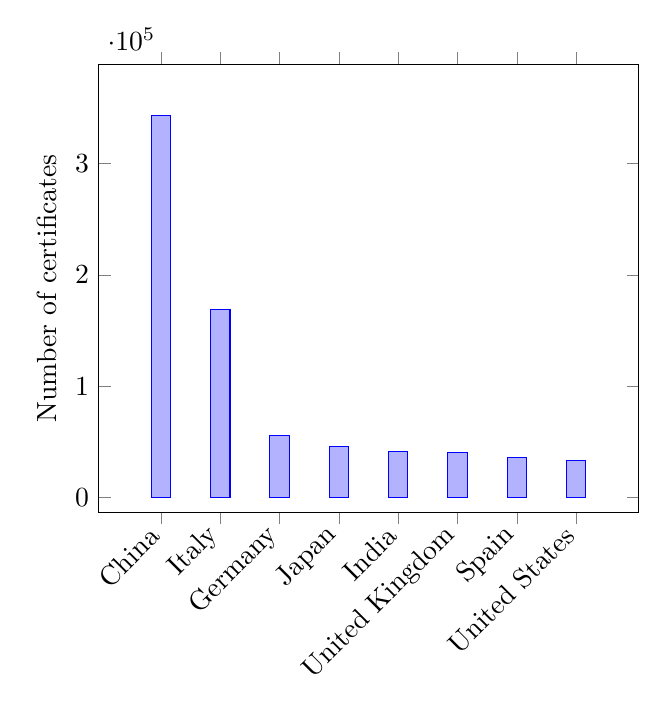
\begin{tikzpicture} \begin{axis}[
    x tick label style={
        /pgf/number format/1000 sep=},
    ylabel= Number of certificates,
    enlargelimits=0.15,
    %legend style={at={(0.5,-0.15)},
        %anchor=north,legend columns=-1},
		symbolic x coords={China, Italy, Germany, Japan, India, United Kingdom, Spain, United States},
		xtick=data,
		x tick label style={rotate=45,anchor=east},
    ybar,
    bar width=7pt,
]
\addplot
    coordinates {(China, 342800) (Italy, 168960)
         (Germany, 55363) (Japan, 45785) (India, 41016)
	(United Kingdom, 40200)	(Spain, 36005) (United States, 33008)};
\end{axis}
\end{tikzpicture}
        		\end{center}
     \end{column}
 \end{columns}
}

\frame{\frametitle{QM-Prozesslandkarte (1)}
\framesubtitle{}
\begin{center}
\includegraphics[width = 10 cm]{Kernprozess} \source{Quelle: Wikimedia/Benji und Markus B\"arlocher}
\end{center}
}

\frame{\frametitle{QM-Prozesslandkarte (2)}
\framesubtitle{}
\begin{center}
\includegraphics[width = 7 cm]{ProzessLK} \source{Quelle: Wikimedia/pz0151}
\end{center}
}



\frame{\frametitle{Elemente des Qualit\"atsmanagementsystem}
\framesubtitle{}
\begin{description}
\item[\textbf{Qualit\"atspolitik}] Absichten und Ausrichtung einer Organisation zu Qualit\"at (durch oberste Leitung ausgedr\"uckt).
\item[\textbf{Qualit\"atsplanung}] Teil des QM, der auf Festlegen der Qualit\"atsziele, Ausf\"uhrungsprozesse und Ressourcen zur Erf\"ullung der Ziele  ausgerichtet ist.
\item[\textbf{Qualit\"atslenkung}]  \"Uberwachung und Korrektur der Realisierung einer Einheit mit dem Ziel, die Qualit\"atsforderungen zu erf\"ullen.
\item[\textbf{Qualit\"atssicherung}] Teil des QM, der darauf ausgerichtet ist, Vertrauen zu erzeugen, dass de Qualit\"atsforderungen erf\"ullt werden.
\item[\textbf{Qualit\"atsverbesserung}]  alle Ma{\ss}nahmen zur Steigerung von Effektivit\"at und Effizienz in T\"atigkeiten und Prozessen.
\end{description}
}

\frame{\frametitle{Beispiel ISO 9000 - Prinzipien}
\framesubtitle{}
\begin{itemize}
\item Kundenorientierung
\item Verantwortlichkeit der F\"uhrung
\item Einbeziehung der beteiligten Personen
\item Prozessorientierter Ansatz
\item Systemorientierter Managementansatz
\item Kontinuierliche Verbesserung
\item Sachbezogener Entscheidungsfindungsansatz
\item Lieferanteneinbeziehung zum gegenseitigen Nutzen
\end{itemize}
}

\frame{\frametitle{ISO 9001 - Ziele}
\framesubtitle{}
\begin{itemize}
\item Vertrauen in Produkte und Dienstleistungen einer Organisation
\begin{itemize}
	\item Konformit\"at
	\item Zuverl\"assigkeit der Ausf\"uhrung
\end{itemize}
\item Kundenzufriedenheit im Fokus
\item Verbesserung der Steuerung der Prozesse
\item Verbesserung des Verst\"andnisses der Prozesse
\item Verbesserung der internen Kommunikation
\end{itemize}
}

\frame{\frametitle{ISO 9001 - Kontext der Organisation}
\framesubtitle{}
\begin{itemize}
\item Verstehen der Organisation und ihres Kontextes
	\begin{itemize}
		\item Bestimmung interner und externer Themen, die f\"ur ihren Zweck relevant sind 
	\end{itemize}
	\item Verstehen der Erfordernisse und Erwartungen interessierter Parteien
	\begin{itemize}
		\item Bestimmung interessierter Parteien f\"ur QMS und deren relevante Anforderungen
	\end{itemize}
	\item Festlegen des Anwendungsbereichs des QMS
	\begin{itemize}
		\item Grenzen und Anwendungsbereich des QMS
		\item Dokumentierte Information:
		\begin{itemize}
		\item Arten der Produkte und Dienstleistungen
		\item Begr\"undung f\"ur Ausschluss
		\end{itemize}
		\item Ausgeschlossene Themen d\"urfen nicht die F\"ahigkeit oder die Verantwortung der Organisation i.S. der Norm beeintr\"achtigen
		\end{itemize}
\end{itemize}
}

\frame{\frametitle{ISO 9001 - Qualit\"atsmanagementsystem und seine Prozesse}
\framesubtitle{}
\begin{itemize}
\item Organisation muss ein QMS aufbauen, aufrechterhalten und fortlaufend verbessern
\item F\"ur QMS ben\"otigte Prozesse bestimmen und Anwendung festlegen
\begin{itemize}
		\item Eingaben und Ergebnisse
		\item Abfolge und Wechselwirkung
		\item Kriterien und Verfahren (inkl. Leistungsindikatoren) f\"ur wirksame Durchf\"uhrung und Steuerung bestimmen und anwenden
		\item Ben\"otigte Ressourcen ermitteln und Verf\"ugbarkeit sicherstellen
		\item Verantwortlichkeiten und Befugnisse zuweisen
		\item Risiken und Chancen behandeln
		\item Prozesse und das QMS verbessern
		\end{itemize}
\item Die Organisation muss dokumentierte Informationen aufrechterhalten, um die Durchf\"uhrung ihrer Prozesse zu unterst\"utzen und die geplante Durchf\"uhrbarkeit der Prozesse zu erm\"oglichen
\end{itemize}
}


\frame[allowframebreaks]{\frametitle{ISO 9001 - Verantwortung der Leitung}
\framesubtitle{}
\begin{itemize}
\item F\"uhrung und Verpflichtung:
	\begin{itemize}
		\item Rechenschaftspflicht
		\item Qualit\"atspolitik und Qualit\"atsziele f\"ur das QMS festlegen (mit Strategie vereinbar)
		\item  Anforderungen des QMS werden in Gesch\"aftsprozesse der Organisation aufgenommen
		\item F\"ordert prozessorientierten Ansatz und risikobasiertes Denken
		\item Sicherstellung von Ressourcenverf\"ugbarkeit
		\item Bedeutung und Wichtigkeit des QMS vermitteln
		\item Personen einsetzen, anleiten und unterst\"utzen, damit diese zur Wirksamkeit des QMS beitragen
		\item Kundenorientierung
	\begin{itemize}
		\item Kunden- und gesetzliche sowie normative Anforderungen erden erf\"ullt
		\item Verbesserung der Kundenzufriedenheit im Fokus
		\item Risiken und Chancen, die Konformit\"at von Produkten und Dienstleistungen beeinflussen k\"onnen, bestimmen und behandeln
	\end{itemize}
	\end{itemize} \newpage
\item Qualit\"atspolitik:
\begin{itemize}
	\item Angemessene Qulit\"atspolitik festlegen (f\"ur Zweck und Kontext der Organisation)
	\item Bietet Rahmen f\"ur Festlegung von Qualit\"atszielen
	\item Verpflichtung zur Erf\"ullung zutreffender Anforderungen (aus ISO 9001) sowie zur fortlaufenden Verbesserung des QMS
	\item Qualit\"atspolitik muss bekanntgemacht werden (als dokumentierte Information)
\end{itemize}
\item Rollen, Verantwortlichkeiten und Befugnisse in der Organisation:
\begin{itemize}
	\item Konformit\"at des QMS mit ISO 9001
	\item Sicherstellung, dass Prozesse die beabsichtigten Ergebnisse liefern
	\item Berichte \"uber Leistung und Verbesserungsm\"oglichkeiten des QMS
	\item F\"orderung der Kundenorientierung
	\item Sicherstellung des QMS bei \"Anderungen
\end{itemize}
\end{itemize}
}

\frame{\frametitle{Planung}
\framesubtitle{}
\begin{columns}[t] 
     \begin{column}[T]{6cm} 
     	\begin{itemize}
     		\item Umgang mit Chancen und Risiken
		\begin{itemize}
		\item Erw\"unschte Auswirkungen verst\"arken
		\item Unerw\"unschte Auswirkungen verhindern
		\end{itemize}
		\item Qualit\"atsziele und deren Erreichung
		\item Planung von \"Anderungen am QMS
     	\end{itemize}
     \end{column}
     	\begin{column}[T]{6cm} 
         	\begin{center}
            		\includegraphics[width=0.8\textwidth]{Risikograf}\source{Quelle: Peter Wratil}
        		\end{center}
     \end{column}
 \end{columns}
}


\frame[allowframebreaks]{\frametitle{ISO 9001 - Unterst\"utzung}
\framesubtitle{}
\begin{itemize}
\item Erforderliche Ressourcen f\"ur Aufbau, Verwirklichung, Aufrechterhaltung und Verbesserung der QMS bestimmen und bereitstellen
\begin{itemize}
	\item F\"ahigkeiten und Beschr\"ankungen von internen Ressourcen
	\item Notwendigerweise extern zu beziehendes
\end{itemize}
\item Personen bestimmen und bereitstellen, die f\"ur Umsetzung des QMS und Betreiben und Steuern der Prozesse n\"otig sind
\item Prozessumgebung (Umgebung f\"ur Durchf\"uhrung der Prozesse und zur Erreichung der Konformit\"at von Produkten und Dienstleistungen):
\begin{itemize}
	\item Soziale, psychologische und physikalische Faktoren
\end{itemize} 
\item Ressourcen zur \"Uberwachung und Messung:
\begin{itemize}
		\item Ressourcen zur Sicherstellung g\"ultiger und zuverl\"assiger \"Uberwachungs- und Messergebnisse
		\item Geeignet f\"ur Art der T\"atigkeit
		\item Aufrechterhaltung der fortlaufenden Eignung
		\item Messtechnische R\"uckf\"uhrbarkeit:
		\begin{itemize}
		\item Kalibrierung gegen nationale oder internationale Normale
		\item Kennzeichnung
		\end{itemize}
		\end{itemize}
\item Wissen der Organisation
\begin{itemize}
		\item Bestimmung des notwendigen Wissens
		\item Aufrechterhaltung des Wissens der Organisation
		\item Anpassung des Wissens der Organisation an sich \"andernde Anforderungen und Entwicklungstendenzen
		\end{itemize}
		\item Kompetenz:
		\begin{itemize}
		\item Erforderliche Kompetenz f\"ur T\"atigkeiten im Zusammenhang mit dem QMS bestimmen
		\item Kompetenz sicherstellen oder erlangen
		\item Angemessene dokumentierte Informationen aufbewahren
		\end{itemize}
\item Bewusstsein der t\"atigen Personen \"uber Qualit\"atspolitik, Qualit\"atsziele, Beitrag zu QMS und Folgen der Nichterf\"ullung
\item Festlegung der Kommunikationswege (intern und extern)
\end{itemize}
}


\frame{\frametitle{ISO 9001 - Lenkung dokumentierter Informationen}
\framesubtitle{}
\begin{itemize}
\item Erstellung und Aktualisierung
\begin{itemize}
	\item Angemessene Kennzeichnung und Beschreibung
	\begin{itemize}
		\item z.B. Titel, Datum, Autor, Referenznummer
	\end{itemize}
	\item angemessenes Format und Medium
	\begin{itemize}
		\item z.B. Sprache, Softwareversion, Grafiken
	\end{itemize}
	\item Angemessene \"Uberpr\"ufung und Genehmigung im Hinblick auf Eignung und Angemessenheit
\end{itemize}
\item Lenkung der Informationen
\begin{itemize}
	\item Informationen sind verf\"ugbar und geeignet
	\item Informationen sind angemessen gesch\"utzt
\end{itemize}
\item Besondere Aufgaben der Dokumentenlenkung
\begin{itemize}
	\item Verteilung, Zugriff, Auffindung und Verwendung
	\item Ablage/Speicherung und Erhaltung (einschlie{\ss}lich Lesbarkeit)
	\item \"Uberwachung von \"Anderungen (z.B. Versionskontrolle)
	\item Aufbewahrung und Verf\"ugung \"uber den weiteren Verbleib
\end{itemize}
\end{itemize}
}

\frame[allowframebreaks]{\frametitle{ISO 9001 - Entwicklung von Produkten% und Dienstleistungen
}
\framesubtitle{}
\begin{itemize}
\item Entwicklungsprozess erarbeiten, umsetzen und aufrechterhalten
\item Entwicklungsplanung
\begin{itemize}
		\item Art, Dauer und Umfang der Entwicklungst\"atigkeiten
		\item Erforderliche Prozessphasen einschlie{\ss}lich \"Uberpr\"ufung der Entwicklung
		\item T\"atigkeiten zur Verifizierung und Validierung
		\item Verantwortlichkeiten und Befugnisse
		\item Internen und externen Ressourcenbedarf
		\item Notwendigkeit der Schnittstellensteuerung
		\item Notwendigkeit der Kunden- und Anwendereinbindung
		\item Anforderungen an Produktion
		\item Steuerungsebene
		\item Dokumentierte Informationen, die die Anforderungserf\"ullung best\"atigen
		\end{itemize}
\item Entwicklungseingaben (angemessen, vollst\"andig und eindeutig)
\begin{itemize}
		\item Funktions- und Leistungsanforderungen
		\item Lessons learned
		\item Gesetzliche und beh\"ordliche Anforderungen
		\item Normen, Standards oder Anleitungen f\"ur die Praxis
		\item M\"ogliche Konsequenzen aus Fehler aufgrund der Art der Produkte
		\item Dokumentierte Informationen \"uber Entwicklungseingaben m\"ussen aufbewahrt werden
		\end{itemize}
\item Steuerungsma{\ss}nahmen f\"ur die Entwicklung
\begin{itemize}
		\item Definition der zu erzielenden Ergebnisse
		\item \"Uberpr\"ufung auf Anforderungsabdeckung
		\item Verifikationsma{\ss}nahmen - Entwicklung er\"ullt Anforderungen aus Entwicklungseingaben
		\item Validierungsma{\ss}nahmen - Entwicklung erf\"ullt Anforderungen aus vorgesehener Anwendung oder dem beabsichtigten Gebrauch
		\item Notwendige Ma{\ss}nahmen aus \"Uberpr\"ufung, Verifikation und Validierung werden umgesetzt
		\item Dokumentierte Informationen \"uber diese T\"atigkeiten aufbewahrt werden
		\end{itemize}
\item Entwicklungs\"anderungen
\begin{itemize}
		\item \"Anderungen im Entwicklungs- oder Produktionsprozess in dem Umfang ermitteln, \"uberpr\"ufen und steuern, der sicherstellt, dass keine nachteilige Auswirkung auf die Konformit\"at mit den Anforderungen entsteht
		\end{itemize} Dokumentierte Informationen
		\begin{itemize}
		\item Entwicklungs\"anderungen
		\item Ergebnisse von \"Uberpr\"ufungen
		\item Autorisierung der \"Anderungen
		\item Eingeleitete Ma{\ss}nahmen zur Vorbeugung nachteiliger Auswirkungen
		\end{itemize}
\end{itemize}
}


\frame{\frametitle{QMS - Umsetzung in der Organisation}
\framesubtitle{}
\begin{columns}[t] 
     \begin{column}[T]{6cm} 
     	\begin{itemize}
     		\item QM-Handbuch: Grunds\"atze, Aufbau- und Ablauforganisation, betriebsweite Zusammenh\"ange, Verantwortungen und Befugnisse
		\item Verfahrensanweisungen: Detaillierte Beschreibung von Teilgebieten des QMS
		\item Arbeits-, Pr\"ufanweisungen etc.: Definition von Einzelt\"atigkeiten, Detailwanweisungen
     	\end{itemize}
     \end{column}
     	\begin{column}[T]{6cm} 
         	\begin{center}
            		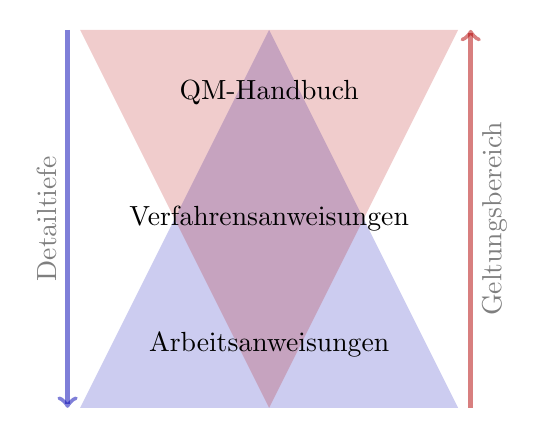
\begin{tikzpicture}[scale = 0.8]
 				\draw[draw = none, fill = blue!70!black, opacity = 0.2] (0,0) -- (3,6) -- (6,0) -- (0,0);
				\draw[draw  = blue!70!black, opacity = 0.5, ->, ultra thick] (-0.2,6) -- (-0.2,0) node[pos = 0.5, rotate = 90, above] {Detailtiefe};
				\draw[draw = none, fill = red!70!black, opacity = 0.2] (0,6) -- (3,0) -- (6,6) -- (0,6);
				\draw[draw  = red!70!black, opacity = 0.5, ->, ultra thick] (6.2,0) -- (6.2,6) node[pos = 0.5, rotate = 90, below] {Geltungsbereich};
				\node at (3,1) {Arbeitsanweisungen};
				\node at (3,3) {Verfahrensanweisungen};
				\node at (3,5) {QM-Handbuch};
			\end{tikzpicture}
        		\end{center}
     \end{column}
 \end{columns}
}

\frame{\frametitle{Auditierung, Zertifizierung und Akkreditierung}
\framesubtitle{}
\begin{itemize}
\item QM-Audit:
\begin{itemize}
		\item Systematische, unabh\"angige Untersuchung
		\item Entsprechen die qualit\"atsbezogenen T\"atigkeiten den geplanten Anordnungen? 
		\item Sind Anordnungen geeignet, die Ziele zu verwirklichen?
		\item Unterscheidung: 
		\begin{itemize}
		\item intern/ extern
		\item System-, verfahrens-, produkt, dienstleistungsorientiert
		\end{itemize}
		\end{itemize}
\item Im Audit wird die Konformit\"at mit Norm festgestellt
\begin{itemize}
		\item Das QM-System wird zertifiziert
		\item Ablauf:
		\begin{itemize}
		\item Autditvorbereitung: Selbstbeurteilung $\rightarrow$ Reife wird beurteilt
		\item Pr\"ufung QM-Handbuch $\rightarrow$ Stichprobe konform?
		\item Audit im Unternehmen $\rightarrow$ Werden beschriebene Abl\"aufe gelebt?
		\item  Zertifikatserteilung
		\end{itemize}
\end{itemize}
\end{itemize}
}

\frame{\frametitle{Branchenspezifische QM-Systeme}
\framesubtitle{Branchenspezifische QMS basieren \"uberwiegend auf der ISO 9001}
\begin{itemize}
\item Automobil:
\begin{itemize}
		\item QS9000 (Nordamerika): branchen- und herstellerspezifische Forderungen
		\item VDA 6 (Deutschland): Erg\"anzend bspw. Prozessf\"ahigkeit, Verf\"ugbarkeit
		\item TS 16949: Vereinheitlichung der verschiedenen Automobil-QMS
\end{itemize}
\item Schienenfahrzeuge:
\begin{itemize}
		\item IRIS (International Railway Industry Standard): Soll Kundenaudits ersetzen, Punktevergabe
		\end{itemize}		
\end{itemize}
}

\frame{\frametitle{Ausblick: Alternative Managementsysteme}
\framesubtitle{Beispiel Capability Maturity Modell Integration (CMMI)}
\begin{columns}[t] 
     \begin{column}[T]{6cm} 
     	\begin{itemize}
     		\item Initial: keine Anforderungen
		\item Managed: Projekte werden gef\"uhrt, ein \"ahnliches Projekt kann erfolgreich wiederholt werden
		\item Defined: angepasster Standardprozess organisationsweite kontinuierliche Verbesserung
		\item Quantitatively Managed: Statistische Prozesskontrolle
		\item Optimizing: Arbeit und Arbeitsweise mittels statistischer Prozesskontrolle verbessert
     	\end{itemize}
     \end{column}
     	\begin{column}[T]{6cm} 
         	\begin{center}
            		\includegraphics[width=0.95\textwidth]{CMMI}\source{Quelle: NASA}
        		\end{center}
     \end{column}
 \end{columns}
}


\frame{\frametitle{Beispiel EG-Konformit\"atserkl\"arung f\"ur Bahnkomponenten \cite{tsilocpas}}
\framesubtitle{}
\begin{columns}[t] 
     \begin{column}[T]{7cm} 
     	\begin{itemize}
     		\item CA: Interne Fertigungskontrolle
		\item CA1: CA + Einzeluntersuchung
		\item CA2: CA + Stichproben
		\item CB: EG-Baumusterpr\"ufung
		\item CC: Bauart-Konformit\"at (interne Fertigungskontrolle)
		\item CD: Bauart-Konformit\"at (QMS f\"ur Produktion)
		\item CF: Konformit\"at (Produktpr\"ufung)
		\item CH: Konformit\"at (vollst\"andiges QMS)
		\item CH1: Konformit\"at (vollst\"andiges QMS) + Enwurfspr\"ufung
     	\end{itemize}
     \end{column}
     	\begin{column}[T]{5cm} 
         	\begin{center}
            		\includegraphics[width=0.95\textwidth]{EGKonformitaet}\source{Quelle: TSI Loc \& Pas}
        		\end{center}
     \end{column}
 \end{columns}
}
